\documentclass{article}

\usepackage[utf8]{inputenc}
\usepackage{xcolor}\usepackage{natbib}
\usepackage{graphicx}
\usepackage{float}
\usepackage{subfig}
\usepackage{blindtext}
\usepackage{hyperref}
\usepackage{setspace}

\setcounter{tocdepth}{3} % Show sections


\newcommand\x{12.7}
\newcommand\y{6}

\graphicspath{{./images/}}
\hypersetup{
    colorlinks=true,
    linkcolor=black,
    filecolor=blue,      
    urlcolor=blue  
    }

% Keywords command
\providecommand{\keywords}[1]
{
  \small	
  \textbf{\textit{Keywords---}} #1
}


\urlstyle{same}

\title{\textbf{Purple Architecture}}
\author{Joris Putteneers}
\date{June 2022}



\begin{document}


\maketitle
% \singlespacing
% \setstretch{1.25}
\tableofcontents
% \newpage

\section{Introduction}
doing normal things stuff the high tech way \cite{databaseII}.\\

enhancing the design proces with smartttech, not the product.
keep the silly design process, intuition, guesswork, imperfect. but enhance it with tech. \\


\keywords{IoAT, machine territories, (in)visible computing, blind systems, artificial naïveté.}

\section{Abstract}
Mario Carpo's description of the “second digital turn” highlights the evolving relationship between the production of knowledge and technological innovations. Anticipating a post-second digital turn focused on the generation of atmospheres and their experiential qualities, this book features scenarios of the extraordinary, fantastic, and the uncanny, whereby deviations from the norm and familiar lend themselves to revealing possibilities for contributing to the development and fostering of emerging, contemporary cultures.



The rapid development of technology and media, where digital and material realities seamlessly blend, provides clarity and opportunities for the future of digital life and spotlights commonplace, contemporary discourses which have become derelict and antiquated. Emerging from this technological revolution are design projects which no longer speculate on possible scenarios but rather aspire for a future rooted in storytelling and world-building. 


The centuries old topic of how to represent reality, and subsequently how to supplant it, anchors these scenarios. In the past few decades, philosophers like Jean Baudrillard, Gilles Deleuze, and Graham Harman, among many others, have all provided insight on experiencing the “real”. The philosophical conundrum was catapulted into western popular culture through the 1999 film, The Matrix. In this film, the character Neo (Keanu Reeves) is faced with a choice between taking a red or blue pill. By consuming the red pill, Neo will awake from a simulation and be introduced to the “real world”, where humans and autonomous machines are at war. By taking the blue pill, he will remain in a simulation, unaware that a parallel environment exists. 


While demanding a radical return to utopian thinking, Zizek speculates on the possibility of a third pill; this book however seeks a heterotopic solution. It questions the assumption that these two conditions are contrary to one another, and rather asks about an option of a purple pill? A reality-virtuality continuum, oscillating between a real environment and one that is virtual, was first introduced in 1994 by Paul Milgram and Fumio Kishino. This concept allowed Milgram and Kishino to contextualize research centered on virtual and augmented reality. But it also contributes to the centuries-old discussion on the creation and reading of representations and images. The purple pill, in the context of this volume, is not reduced to an inbetween hybrid liminal condition. Purpleness is also as ontologically autonomous (and gradient) as any other color on the electromagnetic spectrum of light.


The plot of The Matrix was heavily inspired by Jean Baudrillard's seminal work Simulacra and Simulation (1983) where he introduced the concept of “hyperreality,” representations so realistic they have the capacity to be perceived as real. Both Baudrillard and fellow philosopher and novelist, Umberto Eco, cite the example of Disneyland, a physical location that sanctifies the fantastic while presenting the theme park as a “real” environment. The reconciliation of the “real” and “fantastic” as illustrated in Disneyland is a dated example of a 1950s purpleness. Today these purple experiences are readily available in the form of hybridized environments that contribute to our spatial understanding. {\color{blue}\LaTeX\ text} \\ 

Provocations:

This book is an edited collection of projects and essays that consider a multitude of purple futures addressing topics such as spatial mediation, the right to space in the (un)built environment, socio-ecological connections, atmosphere making, and virtual realms. The content operates within varying scales, time periods, degrees of physicality and virtuality, while implementing technological innovations for aspirational outputs.


The book offers the following provocations but can be expanded to include other examples of purpleness:

What qualities constitute a purple condition in a spatial experience?

What processes, mediums, and agents are involved in worldbuilding that consists of purple qualities and characteristics?

How do purple qualities assist in responding to the climatic and socio-political crisis that we face today?

How do purple qualities contribute to the atmosphere and experience of a spatial condition?


Please note that this book is about design and theory, discourse and dialogue, and therefore technical descriptions, quantitative studies, and pedagogical/curricular research evaluating student performance are outside the scope of the book.



\begin{figure}[H]
  \centering
  % \captionsetup{}
  \captionsetup{font=small,justification=raggedright,singlelinecheck=false}
  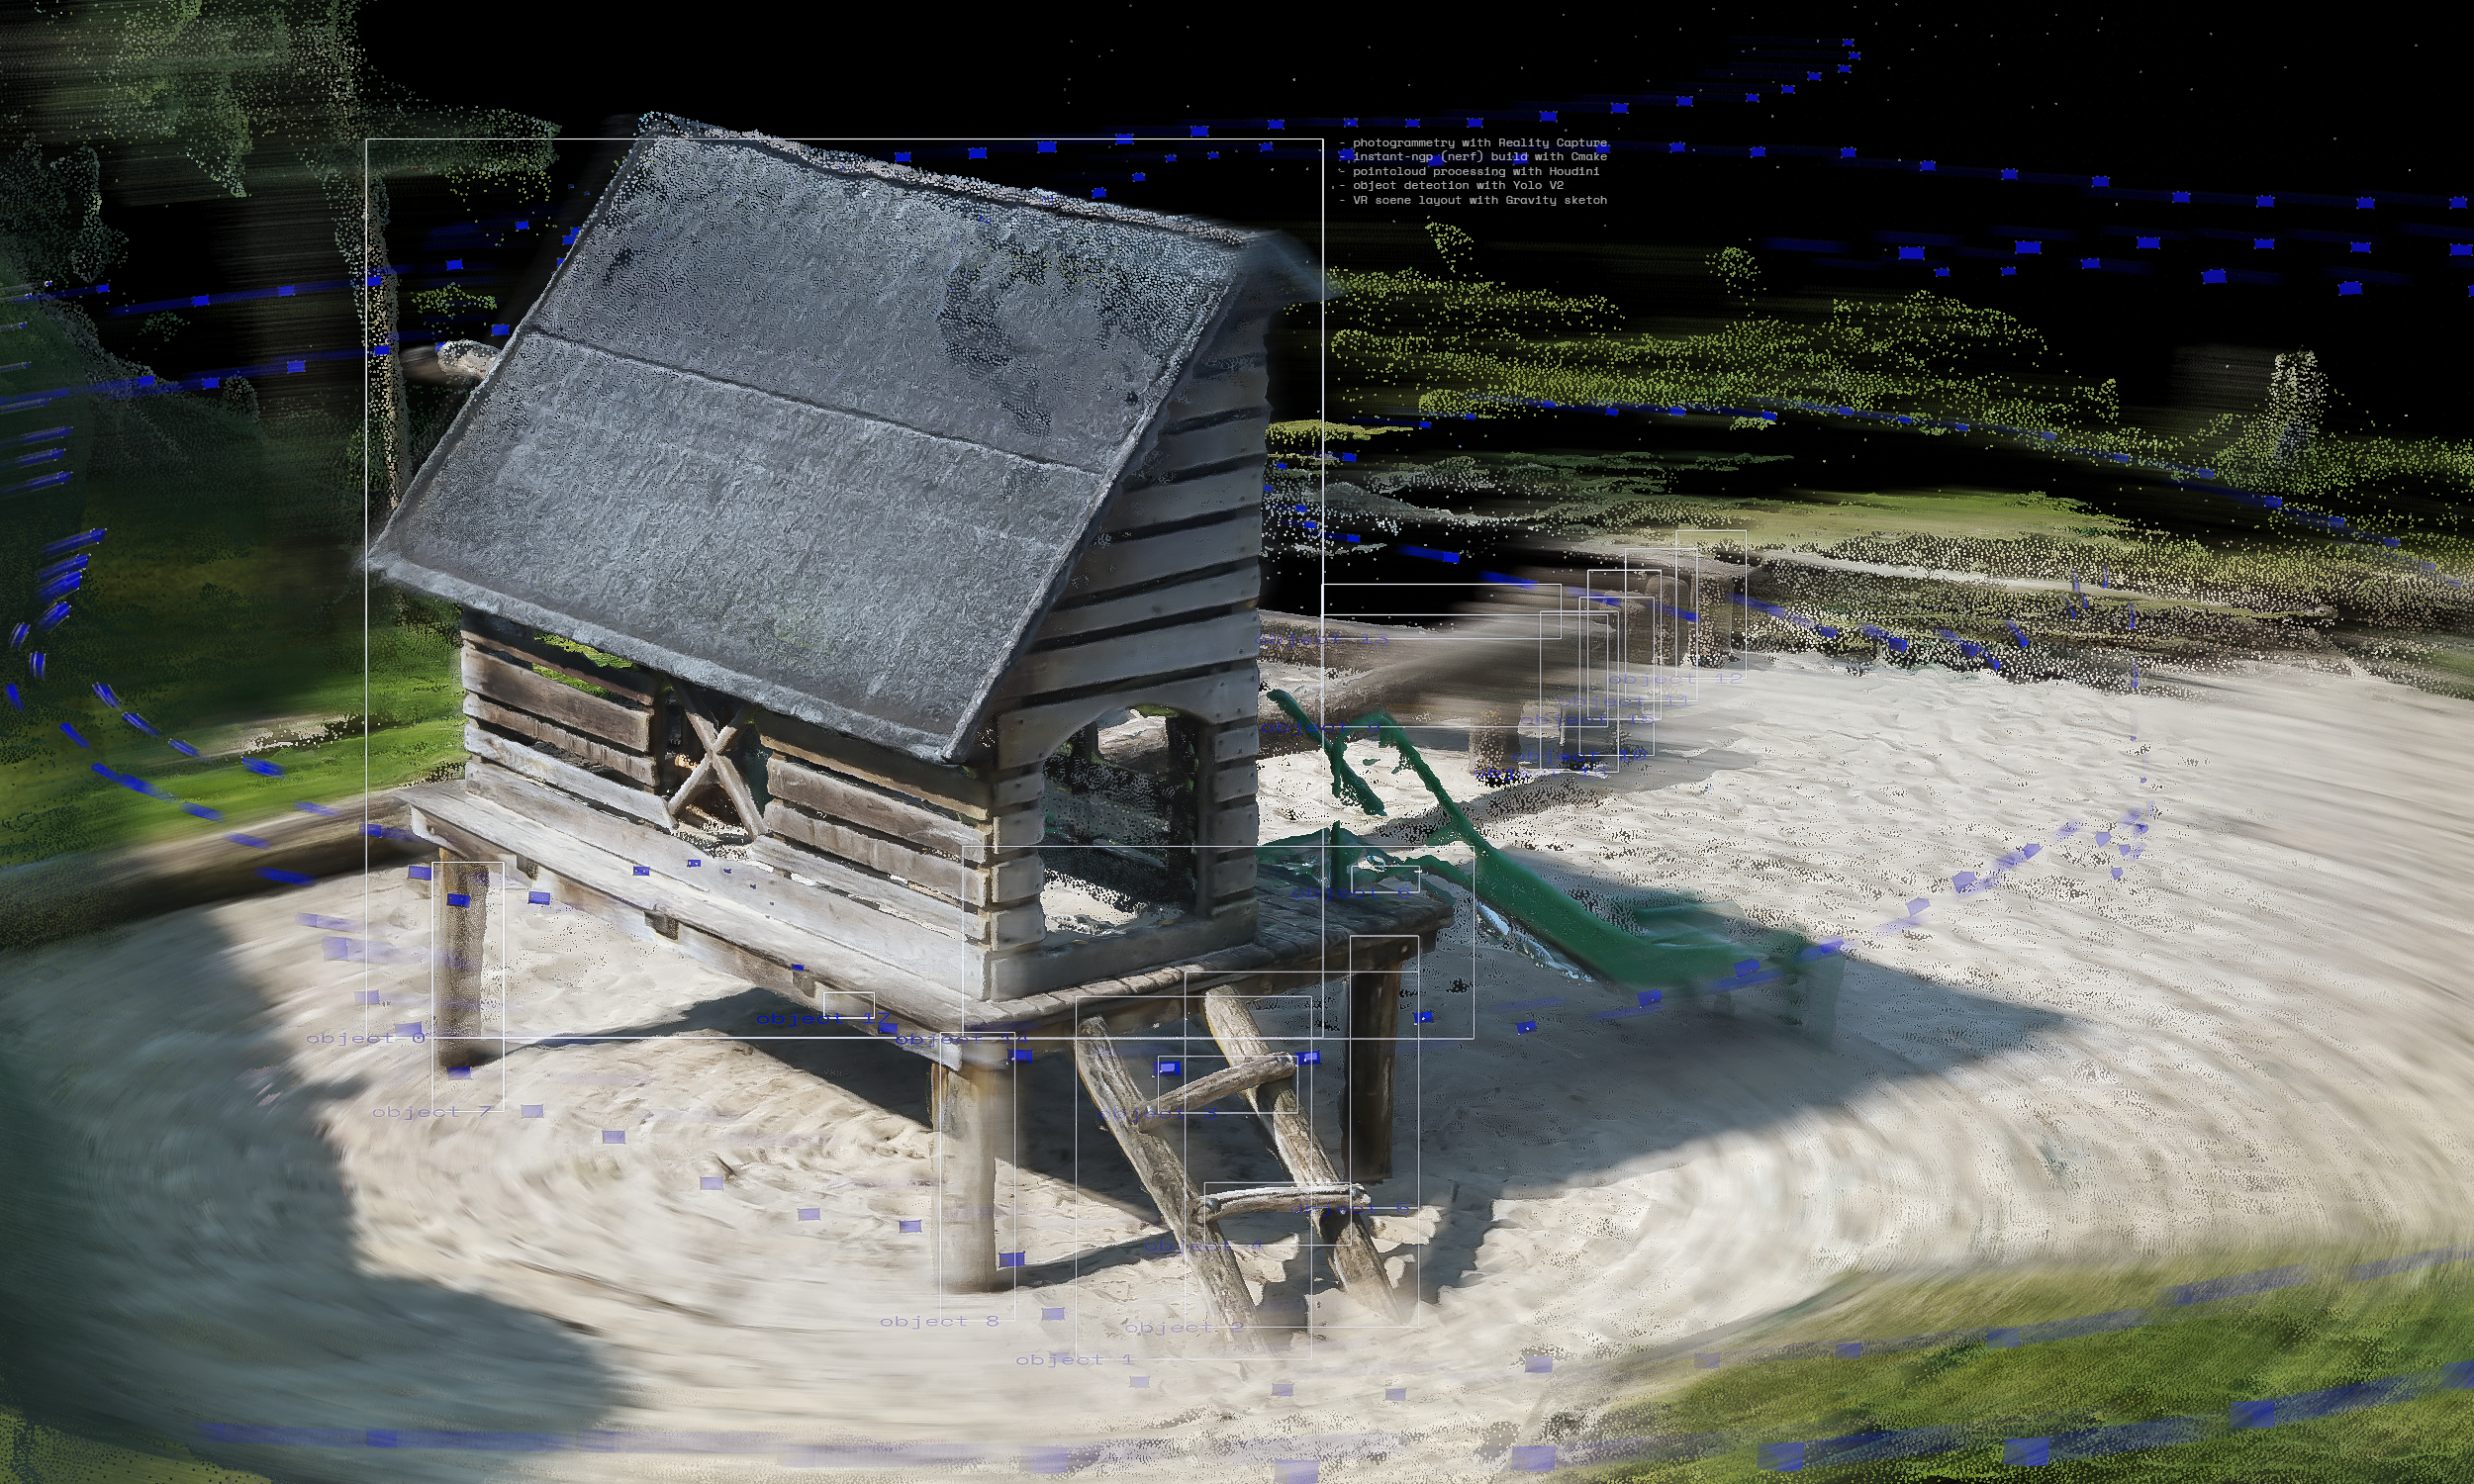
\includegraphics[width=\x cm]{g.png}
  \caption{pointcloud model. \href{https://sketchfab.com/3d-models/wifi-workspace-visualisation-aefe16a1f9bd4296941e099754eaacc2}{sketchfab Model}.}
  \label{fig:method}
\end{figure}


\begin{figure}[H]
  \centering
  % \captionsetup{}
  \captionsetup{font=small,justification=raggedright,singlelinecheck=false}
  \includegraphics[width=\x cm]{c.png}
  \caption{pointcloud model. \href{https://sketchfab.com/3d-models/wifi-workspace-visualisation-aefe16a1f9bd4296941e099754eaacc2}{sketchfab Model}.}
  \label{fig:method}
\end{figure}

\begin{figure}[H]
  \centering
  % \captionsetup{}
  \captionsetup{font=small,justification=raggedright,singlelinecheck=false}
  \includegraphics[width=\x cm]{a.jpg}
  \caption{pointcloud model. \href{https://sketchfab.com/3d-models/wifi-workspace-visualisation-aefe16a1f9bd4296941e099754eaacc2}{sketchfab Model}.}
  \label{fig:method}
\end{figure}





\begin{figure}[H]
  % \centering
  \captionsetup{font=small,justification=raggedright,singlelinecheck=false}
  \parbox{6cm}{
  \includegraphics[width=\y cm]{b.png}
  % \captionsetup{font={small,sc,onehalfspacing,color=red}}
  \caption{Object detection.}
  \label{fig:2figsA}}
  \qquad
  \begin{minipage}{6cm}
  \includegraphics[width=\y cm]{a.png}
  \caption{Machine vision iteration.}
  \label{fig:2figsB}
  \end{minipage}
\end{figure}

\begin{figure}[H]
  % \centering
  \captionsetup{font=small,justification=raggedright,singlelinecheck=false}
  \parbox{6cm}{
  \includegraphics[width=\y cm]{h.png}
  % \captionsetup{font={small,sc,onehalfspacing,color=red}}
  \caption{Object detection.}
  \label{fig:2figsA}}
  \qquad
  \begin{minipage}{6cm}
  \includegraphics[width=\y cm]{i.png}
  \caption{Machine vision iteration.}
  \label{fig:2figsB}
  \end{minipage}
\end{figure}



\section{Section}
Dummy text
\subsection{Subsection}
Dummy text



\section{Author}
Joris putteneers is an architect and researcher, interested in speculating the anthroposcene through means of software, hardware and media technologies.\\
\\ 
His work has been exhibited at MomA New York, Londen design festival, Venice Biennale and multiple film festivals. He has taught studios and workshops internationally at the Bartlett UCL, Texas A\&M, KUL Faculty of Architecture and TU Wien. Since 2017 he has been actively working in his practice where he develops software and hardware solutions in the fields of Data driven architectural design, vision systems and architectural representation. Currently he is working as a researcher at the KUL Faculty of Architecture developing interdiscpilinairy curricula for Engineers, Architects and Artists. \\





\section{Conclusion}
``I always thought something was fundamentally wrong with the universe'' \citep{adams1995hitchhiker}\\
DSFdsfdsFfdsfdsfdffsfdsfdf

\bibliographystyle{plain}
% \bibliography{references}
\end{document}